Como se comentó en el capítulo~\ref{cap:Objetivo}, la optimización se va a resolver como un \textbf{problema de satisfacción de restricciones}.\\

La programación por restricciones es una metodología software que permite resolver problemas de gran complejidad, típicamente NP. Un \gls{PSR}~\cite{Russ06} está caracterizado por:
\begin{itemize}
	\item Un conjunto de variables, donde cada variable dispone de un dominio de valores que puede tomar.
	\item Un conjunto de restricciones, que permite conocer las posibles combinaciones de las variables.
	\item La solución al PSR será la asignación de valores a las variables de forma que se satisfacen las restricciones y se alcanza el objetivo, representado típicamente como una función a optimizar.
\end{itemize}

\subsection{Variables del PSR}

El objetivo del problema es obtener valores de energía para los paneles fotovoltaicos, baterías y red eléctrica, de tal modo que se cubra la demanda energética del hogar y que el gasto económico sea el menor. Es por esto que las variables propias del problema de satisfacción de restricciones serán:
\begin{itemize}
\item \textbf{Energía fotovoltaica (EF)}. Energía obtenida de los módulos fotovoltaicos.
\item \textbf{Energía de red (ER)}. Energía importada de la red eléctrica.
\item \textbf{Energía de batería (EB)}. Energía obtenida de la batería.
\item \textbf{Consumo de batería (CB)}. Energía consumida para cargar la batería.
\item \textbf{Consumo de red (CR)}. Energía vertida a red a cambio de retribución económica.
\end{itemize}
En la Tabla~\ref{tab:domains} se muestran los dominios de estas variables.
\begin{table}[H]
        \centering
        \begin{tabular}{|c|c|}
        \hline
         \textbf{Variable del PSR} & \textbf{Dominio}\\ \hline
          Energía fotovoltaica (\gls{EF}) & $ Dom_{EF} = [0, EF_{max}] $ \\ \hline
          Energía de red (\gls{ER}) & $ Dom_{ER} = [0, +\infty) $\\ \hline
          Energía de batería (\gls{EB}) & $ Dom_{EB} = [0, +\infty) $\\ \hline
          Consumo de batería (\gls{CB}) & $ Dom_{CB} = [0, +\infty) $\\ \hline
          Consumo de red (\gls{CR}) & $ Dom_{CR} = [0, +\infty) $\\ \hline
        \end{tabular}
        \caption{Dominios de las variables del PSR}
        \label{tab:domains}
\end{table}

Las restricciones estarán definidas en función de dichas variables y cada solución al problema estará formada por un valor para cada una de estas variables. Estos valores satisfacen las restricciones y además serán los óptimos para que se produzca el menor gasto económico posible. El resto de variables (variables de control) determinarán las propias restricciones y el valor de las anteriores dependerá de éstas en una hora concreta t, entre 0 y 24h.\\

\subsection{Restricciones del PSR}
A continuación se determinan las restricciones a las que está sometido el modelo en una hora t:
\begin{itemize}
\item \textbf{Toda la energía generada debe ser consumida} (~\ref{eq:restr1}).\\ \\Hace referencia al principio básico de la energía, la energía que se produce se consume de un modo u otro, no es posible que la suma de las variables correspondientes a la generación de energía (EB, ER y EF) sea distinta a la suma de las variables que hacen referencia al consumo de energía (CR, CB, $ C_{int} $ y C). Esto debe producirse en cada una de las horas de la simulación. Así, tenemos una restricción lineal y n-aria correspondiente a las 24 horas correspondientes a una simulación, por lo que ésta restricciones a efectos prácticos es tomada como 24 restricciones a cumplir.
\begin{equation}
        \label{eq:restr1}
        \forall_{i} \in [0, 1, 2, ..., 24) : EF_{i}+ER_{i}+EB_{i} = CR_{i}+CB_{i}+C_{int}+C
\end{equation}

\item \textbf{No se puede producir energía fotovoltaica durante la noche} (~\ref{eq:restr2}).\\ \\Algo obvio, pues sin luz solar la energía fotovoltaica no es posible. Esto no está controlado en la API AEMET, ya que las peticiones relativas a la noche no reflejan una descripción propia del tiempo nocturno, si no que devuelve los mismos valores independientemente de si existe luz solar, por lo que debe manejarse mediante una restricción. Para este trabajo las horas de la noche serán las pertenecientes al intervalo temporal desde las 22:00 pm hasta las 7:00 am. Como posible trabajo futuro, podría determinarse este intervalo en función de la estación del año para que pueda ser un intervalo con mayor grado de efectividad. Se trata de una restricción unaria, donde para ciertos valores de t, EF debe ser 0. Es por esto que esta restricción a efectos prácticos es tomada como nueve restricciones (las nueve horas de noche definidas anteriormente)
\begin{equation}
        \label{eq:restr2}
        EF_{noche} = 0
\end{equation}

\item \textbf{La energía fotovoltaica generada no puede ser mayor que la máxima energía fotovoltaica en t} (~\ref{eq:restr3}).\\ \\No se puede superar el umbral de generación de energía fotovoltaica establecido por la potencia nominal máxima de esa hora t, pues se estaría violando la capacidad real de producción de los módulos fotovoltaicos del sistema. Es una restricción lineal unaria, ya que la energía fotovoltaica máxima de cada hora t es constante, pues como se comentó anteriormente, sólo es dependiente del número de módulos fotovoltaicos y la situación meteorológica (obtenida de la API AEMET). A efectos prácticos, esta restricción es tomada como 24 restricciones a cumplir referentes a las 24 horas de la simulación.
\begin{equation}
        \label{eq:restr3}
        \forall_{i} \in [0, 1, 2, ..., 24) : EF_{i} \leq EF_{i}^{max}
\end{equation}

\item \textbf{La energía obtenida de la batería no puede ser mayor que el nivel de batería actual teniendo en cuenta la profundidad máxima de descarga} (~\ref{eq:restr4}).\\ \\Básicamente no se puede obtener una cantidad de energía mayor a la posible en esa hora t, que vendrá determinada por la diferencia entre el  nivel de carga disponible al comienzo de esa hora y la capacidad máxima de la batería por la profundidad de descarga (50\%), para evitar daños en su ciclo de vida útil. Restricción unaria, pues solo involucra la variable EB, ya que el resto de elementos de la restricción son constantes en una hora t (nivel de carga actual, capacidad máxima de la batería y profundida de descarga). Al igual que las restricciones anteriores es lineal y a efectos prácticos representa 24 restricciones a cumplir.
\begin{equation}
        \label{eq:restr4}
        \forall_{i} \in [0, 1, 2, ..., 24) : EB_{i} \leq nivel_{i-1} - capacidad_{max} * profundidad_{descarga}
\end{equation}

\item \textbf{El consumo para cargar la batería no puede ser mayor que la capacidad de la misma menos el nivel restante después de t} (~\ref{eq:restr5}).\\Parecido a la restricción anterior, en esta se modela el hecho de cargar la batería (CB) en cada hora t, el cuál está condicionado por la cantidad de batería restante para completar la carga (100\%), obtenido mediante la diferencia entre la capacidad máxima de la misma y lo consumido en la hora t (nivel de carga antes de comenzar la hora t menos la energía consumida de batería en t). Restricción binaria pues involucra tanto el consumo de batería (CB) como la energía de batería (EB), siendo la capacidad máxima de la batería y el nivel de carga en t constantes. Es tomado como 24 restricciones ya que debe cumplirse en cada una de las 24 horas de una simulación.
\begin{equation}
        \label{eq:restr5}
        \forall_{i} \in [0, 1, 2, ..., 24) : CB_{i} \leq capacidad_{max}- (nivel_{i-1} - EB_{i})
\end{equation}

\end{itemize}

Por lo tanto, a efectos prácticos, el PSR tiene 81 restricciones que satisfacer para determinar los valores de las variables.

\subsection{Función Objetivo}
Cómo se ha comentado antes, un problema de satisfacción de restricciones está determinado por un conjunto de variables y sus dominios, un conjunto de restricciones sobre esas variables y un objetivo. Por el momento se dispone de los dos primeros, por lo que en este apartado se procede a determinar el último, \textbf{la función objetivo}.\\

Un PSR que cuenta únicamente con variables y restricciones para esas variables podrá tener numerosas soluciones, representadas como una tupla con valores para cada variable. Añadiendo un objetivo al PSR se consigue unificar la solución, pues de todas esas soluciones, sólo una optimizará un objetivo concreto, y contendrá los valores óptimos de cada variable para ello.\\

Como se ha comentado a lo largo del desarrollo de este \gls{TFG}, el objetivo del problema es \textbf{minimizar el gasto económico} producido mediante la optimización de energía en cada simulación de 24 horas, por lo tanto se buscarán valores de las variables que, además de satisfacer el conjunto de restricciones, sean óptimos para que el gasto económico sea mínimo. Éste gasto económico es dependiente del precio en la hora t de cada una de las energías que representan las variables. De estos precios se habló y se implementó la forma de obtenerlos en la Iteración~\ref{sec:hito1}. Sus valores son constantes en cada hora t. Dicho esto, la función objetivo a minimizar está formada por el sumatorio de los costos económicos en cada hora t, por lo que representa el gasto económico de toda la simulación (~\ref{eq:funcionObjetivo}).
\begin{equation}
\label{eq:funcionObjetivo}
f(x) = \sum_{i=0}^{23} EF_{i}P_{i}^{F} + ER_{i}P_{i}^{R_{PVPC}} + EB_{i}P_{i}^{B_{out}} - CB_{i}P_{i}^{B_{in}} - CR_{i}P_{i}^{R_{SPOT}}
\end{equation}
Siendo:
\begin{itemize}
\item $ EF_{i}P_{i}^{F} $: Gasto económico producido al generar energía fotovoltaica en la hora t.
\item $ ER_{i}P_{i}^{R_{PVPC}} $: Gasto económico producido al importar energía a la compañía eléctrica en la hora t.
\item $ EB_{i}P_{i}^{B_{out}} $: Gasto económico producido al descargar la batería en la hora t.
\item $ CB_{i}P_{i}^{B_{in}} $: Ganancia económica producida al cargar la batería en la hora t.
\item $ CR_{i}P_{i}^{R_{SPOT}} $: Ganancia económica producida al verter energía al mercado eléctrico en la hora t.
\end{itemize}

En cada simulación se buscará que el valor de $ f(x) $ sea el menor posible y la solución al PSR de esa simulación son los valores que deben tomar las variables para hacerlo posible.

\subsection{Implementación de la clase Simulation}
Vistos los apartados anteriores, es la hora de implementar una clase para representar el modelo de simulación y poder crear objetos que representan una simulación concreta. Esta clase se llama \textbf{Simulation} (Figura~\ref{fig:simulation} y está disponible en el módulo simulation. Los atributos de la clase Simulation serán las variables de control que tendrá cada objeto correspondiente a una simulación:
\begin{itemize}
        \item start: variable de control relativa a la fecha de inicio de la simulación. Es de tipo datetime.
        \item end: variable de control relativa a la fecha de fin de la simulación. Al igual que start, es una variable de formato fecha (datetime).
        \item ef\_price: variable de control referente al precio de generar energía fotovoltaica. Se trata de un número tipo float, pues tendrá el mismo valor en toda la simulación (se obtiene a partir de la inversión realizada).
        \item er\_price: variable de control referente a los precios que tendrá el \gls{PVPC} en cada hora de la simulación. Es una lista de 24 elementos de tipo float.
        \item eb\_price: variable de control referente al precio de descargar la batería. Es un número de tipo float ya que será igual en las 24 horas de la simulación.
        \item cr\_price: variable de control referente a los precios SPOT en cada hora de la simulación, es decir, el precio del vertido de energía a la red eléctrica.
        \item cb\_price: variable de control referente a los precios de cargar la batería. Como es dependiente de los precios de energía fotovoltaica y de red de cada hora t, se trata de una lista con 24 valores.
        \item battery\_capacity: variable de control referente a la capacidad total de la batería. Variable de tipo float.
        \item battery\_level: variable de control que representa el nivel inicial de carga de la batería. Variable de tipo float.
        \item discharge\_depth: variable de control referente a la profundidad de descarga permitida en la batería. Variable de tipo float.
        \item max\_ef\_buffer: Más que una variable de control, representa los 24 valores máximos posibles de energía fotovoltaica, obtenidos como se comentó anteriormente mediante la información de la API AEMET y el número de módulos fotovoltaicos, por tanto, se trata de una lista de 24 valores.
        \item c\_int: referente a la variable de control del consumo interno del sistema. Variable de tipo float.
        \item c: referente al consumo del hogar, lista de los 24 valores con el consumo del hogar en las 24 horas de la simulación.

Las funciones de esta clase sirven para calcular algunos de los atributos anteriores. En la Figura~\ref{fig:simulation} se muestra la clase UML de Simulation.
\end{itemize}

\begin{figure}[H]
        \centering
        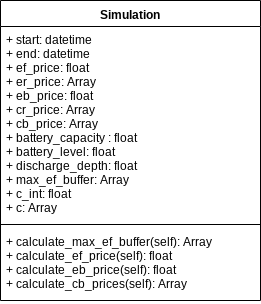
\includegraphics[width=6cm]{figs/simulation_class.png}
        \caption{Clase Simulation}
        \label{fig:simulation}
\end{figure}

En la próxima iteración se implementará cada una de las restricciones para ejecutar la simulación.
